\chapter{Traffic Signals}

Traffic signals are part of our daily life and it is very important to teach about it to children for their safety and to make them a responsible citizen. This project, built as a model of traffic signals by using LEDs, can be used to teach the basics of road safety to children.

\subsection*{Components}
\begin{table}[H]
    \centering
    \begin{tabular}{|c|l|c|}\hline
     \textbf{\#} & \textbf{Components} &  \textbf{Amount}\\\hline
     1 & Red LED                & 4 \\\hline
     2 & Green LED              & 4 \\\hline
     3 & Yellow LED             & 4 \\\hline
     4 & 470 $\Omega$ resistor   & 11 \\\hline
     5 & Arduino UNO            & 1 \\\hline
     6 & Connecting wires       & - \\\hline
    \end{tabular}
\end{table}

\subsection*{Connections}

\begin{enumerate}[leftmargin=*]
    \item Connect 470 $\Omega$ resistors with the anode of all LEDs except those which are to be connected to pin 13 of Arduino.
    \item Connect the other end of the resistors of all LEDs to pin 2-13 of Arduino.
    \item Connect the cathodes of all LEDs to GND of Arduino.
\end{enumerate}

Fig. \ref{fig:traffic} illustrates the connections of the components.
	
\subsection*{Procedure}
\begin{enumerate}[leftmargin=*]
     \item Copy lst. \ref{list:traffic-signals} to a new Arduino sketchbook. Upload the code to your Arduino board.
    \item Observe the working of traffic signals. 
    
\end{enumerate}

\begin{figure}[H]
	\centering 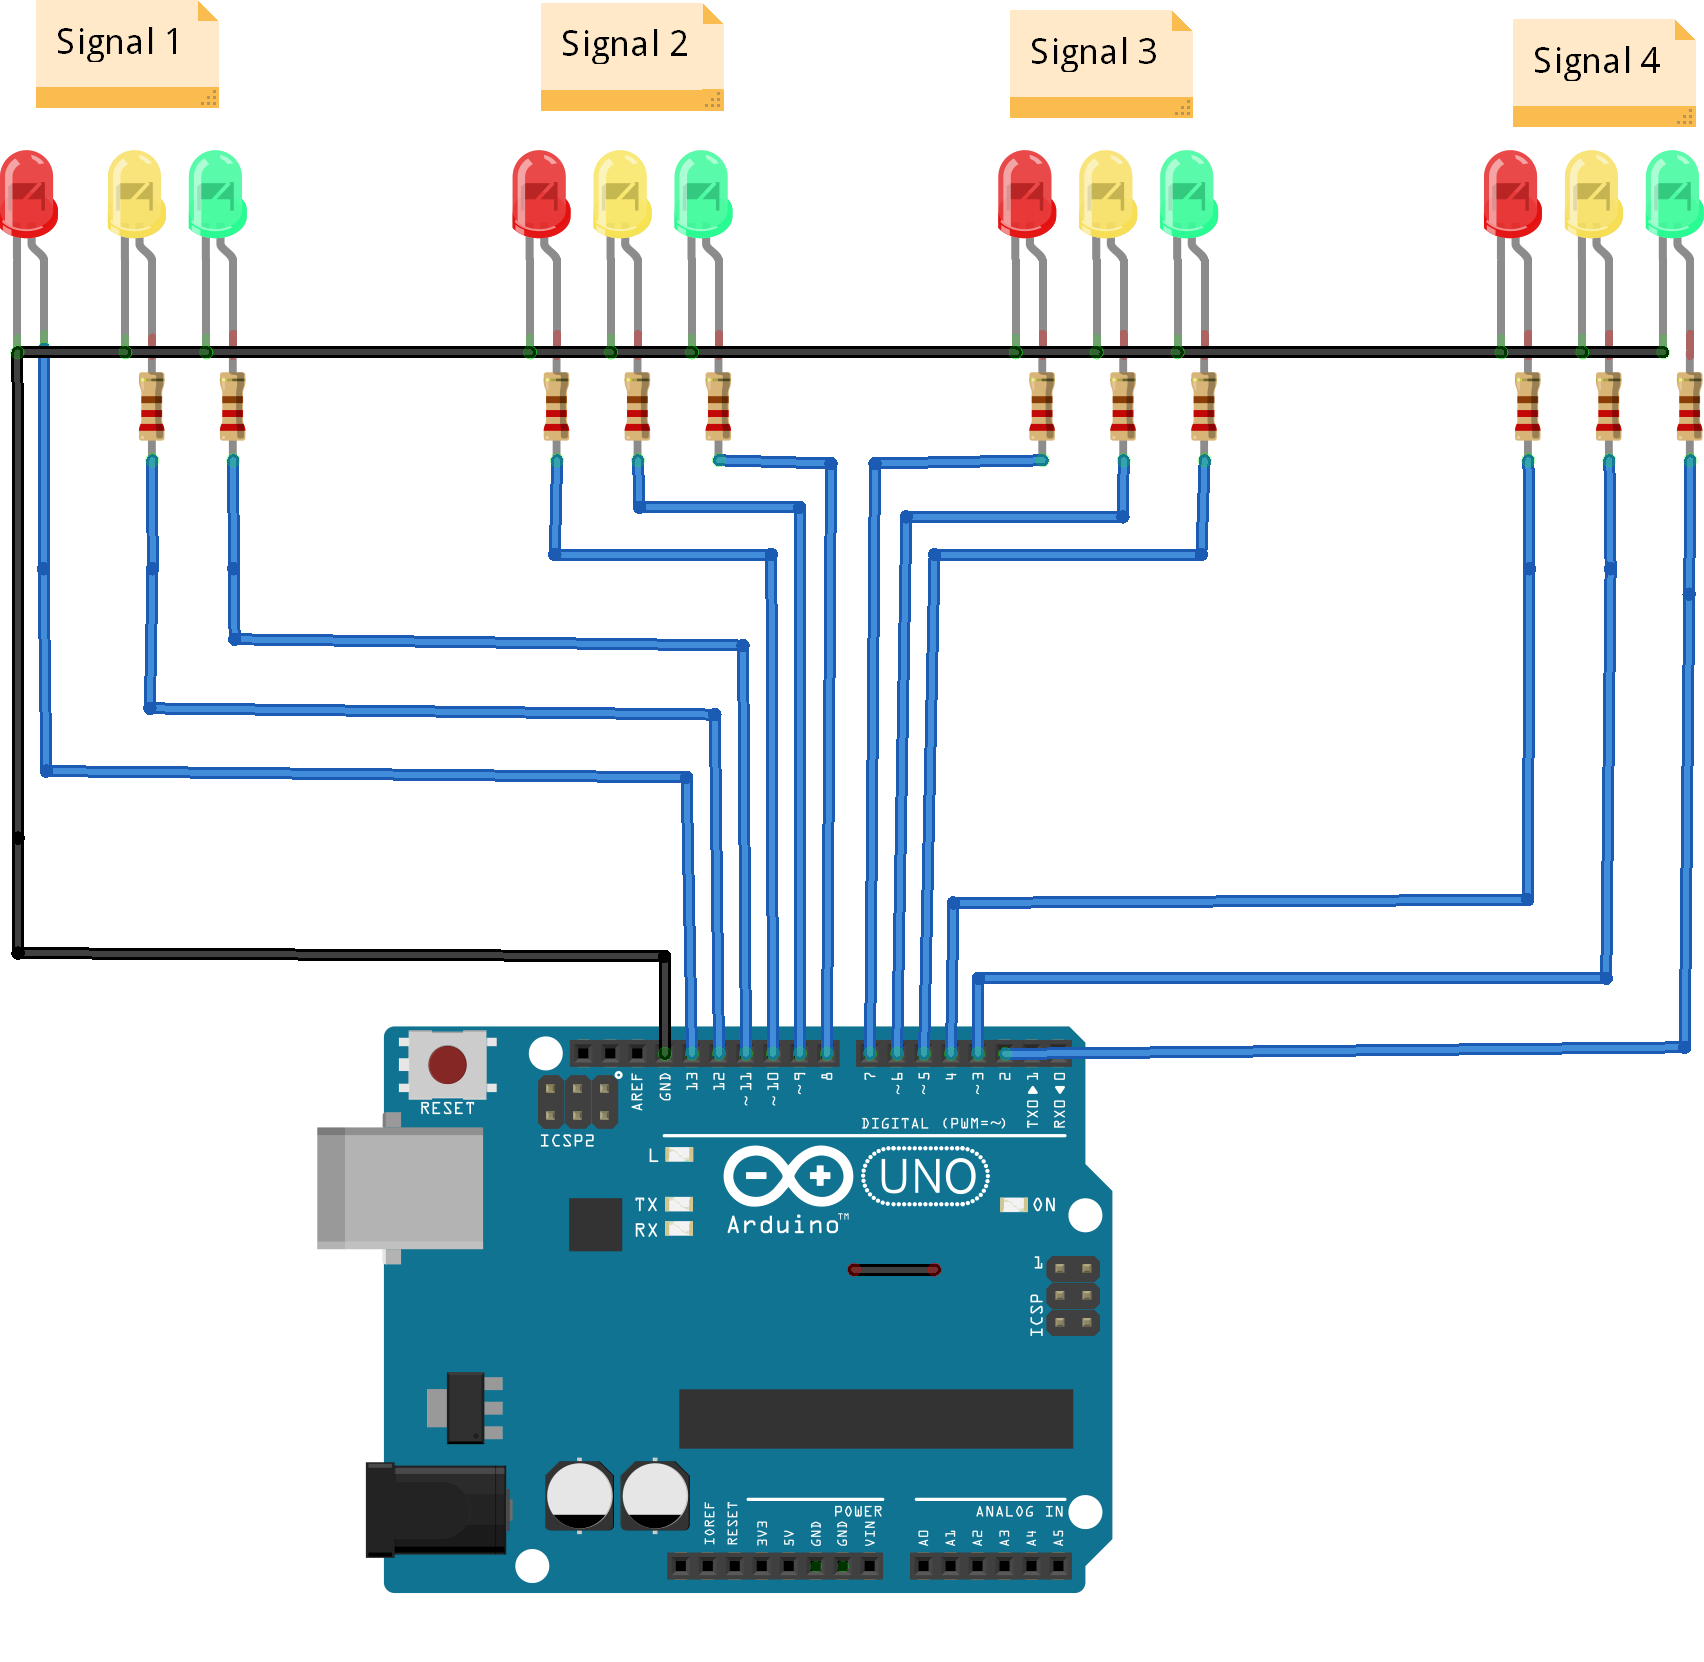
\includegraphics[width=0.5\linewidth]{Figures/recreational_exp/traffic light_bb.png}
	\caption{Circuit diagram}
	\label{fig:traffic}
	\end{figure}
	
\begin{lstlisting}[language=Arduino, numbers=none, caption={Code for generating signals for traffic lights}, captionpos=b, label={list:traffic-signals}]
int r1=4;
int y1=3;
int g1=2;

int r2=7;
int y2=6;
int g2=5;

int r3=10;
int y3=9;
int g3=8;

int r4=13;
int y4=12;
int g4=11;

void setup() {
  // put your setup code here, to run once:
    pinMode(r1, OUTPUT);
    pinMode(y1, OUTPUT);
    pinMode(g1, OUTPUT);
    
    pinMode(r2, OUTPUT);
    pinMode(y2, OUTPUT);
    pinMode(g2, OUTPUT);
    
    pinMode(r3, OUTPUT);
    pinMode(y3, OUTPUT);
    pinMode(g3, OUTPUT);
    
    pinMode(r4, OUTPUT);
    pinMode(y4, OUTPUT);
    pinMode(g4, OUTPUT);
}

void trafic_signal (int r,int  y, int g)
{
    digitalWrite(r, HIGH);
    digitalWrite(y, LOW);
    digitalWrite(g, LOW);
    delay(6000);
    digitalWrite(r, LOW);
    digitalWrite(y, HIGH);
    delay(10);
    digitalWrite(y, LOW);
    digitalWrite(g, HIGH);
    delay(2000);
    digitalWrite(g, LOW);
}

void loop() {
    // put your main code here, to run repeatedly:

    trafic_signal(r1,y1,g1); // signal 1
    trafic_signal(r2,y2,g2); // signal 2
    trafic_signal(r3,y3,g3); // signal 3
    trafic_signal(r4,y4,g4); // signal 4
}
\end{lstlisting}

\begin{figure}[H]
	\centering 
	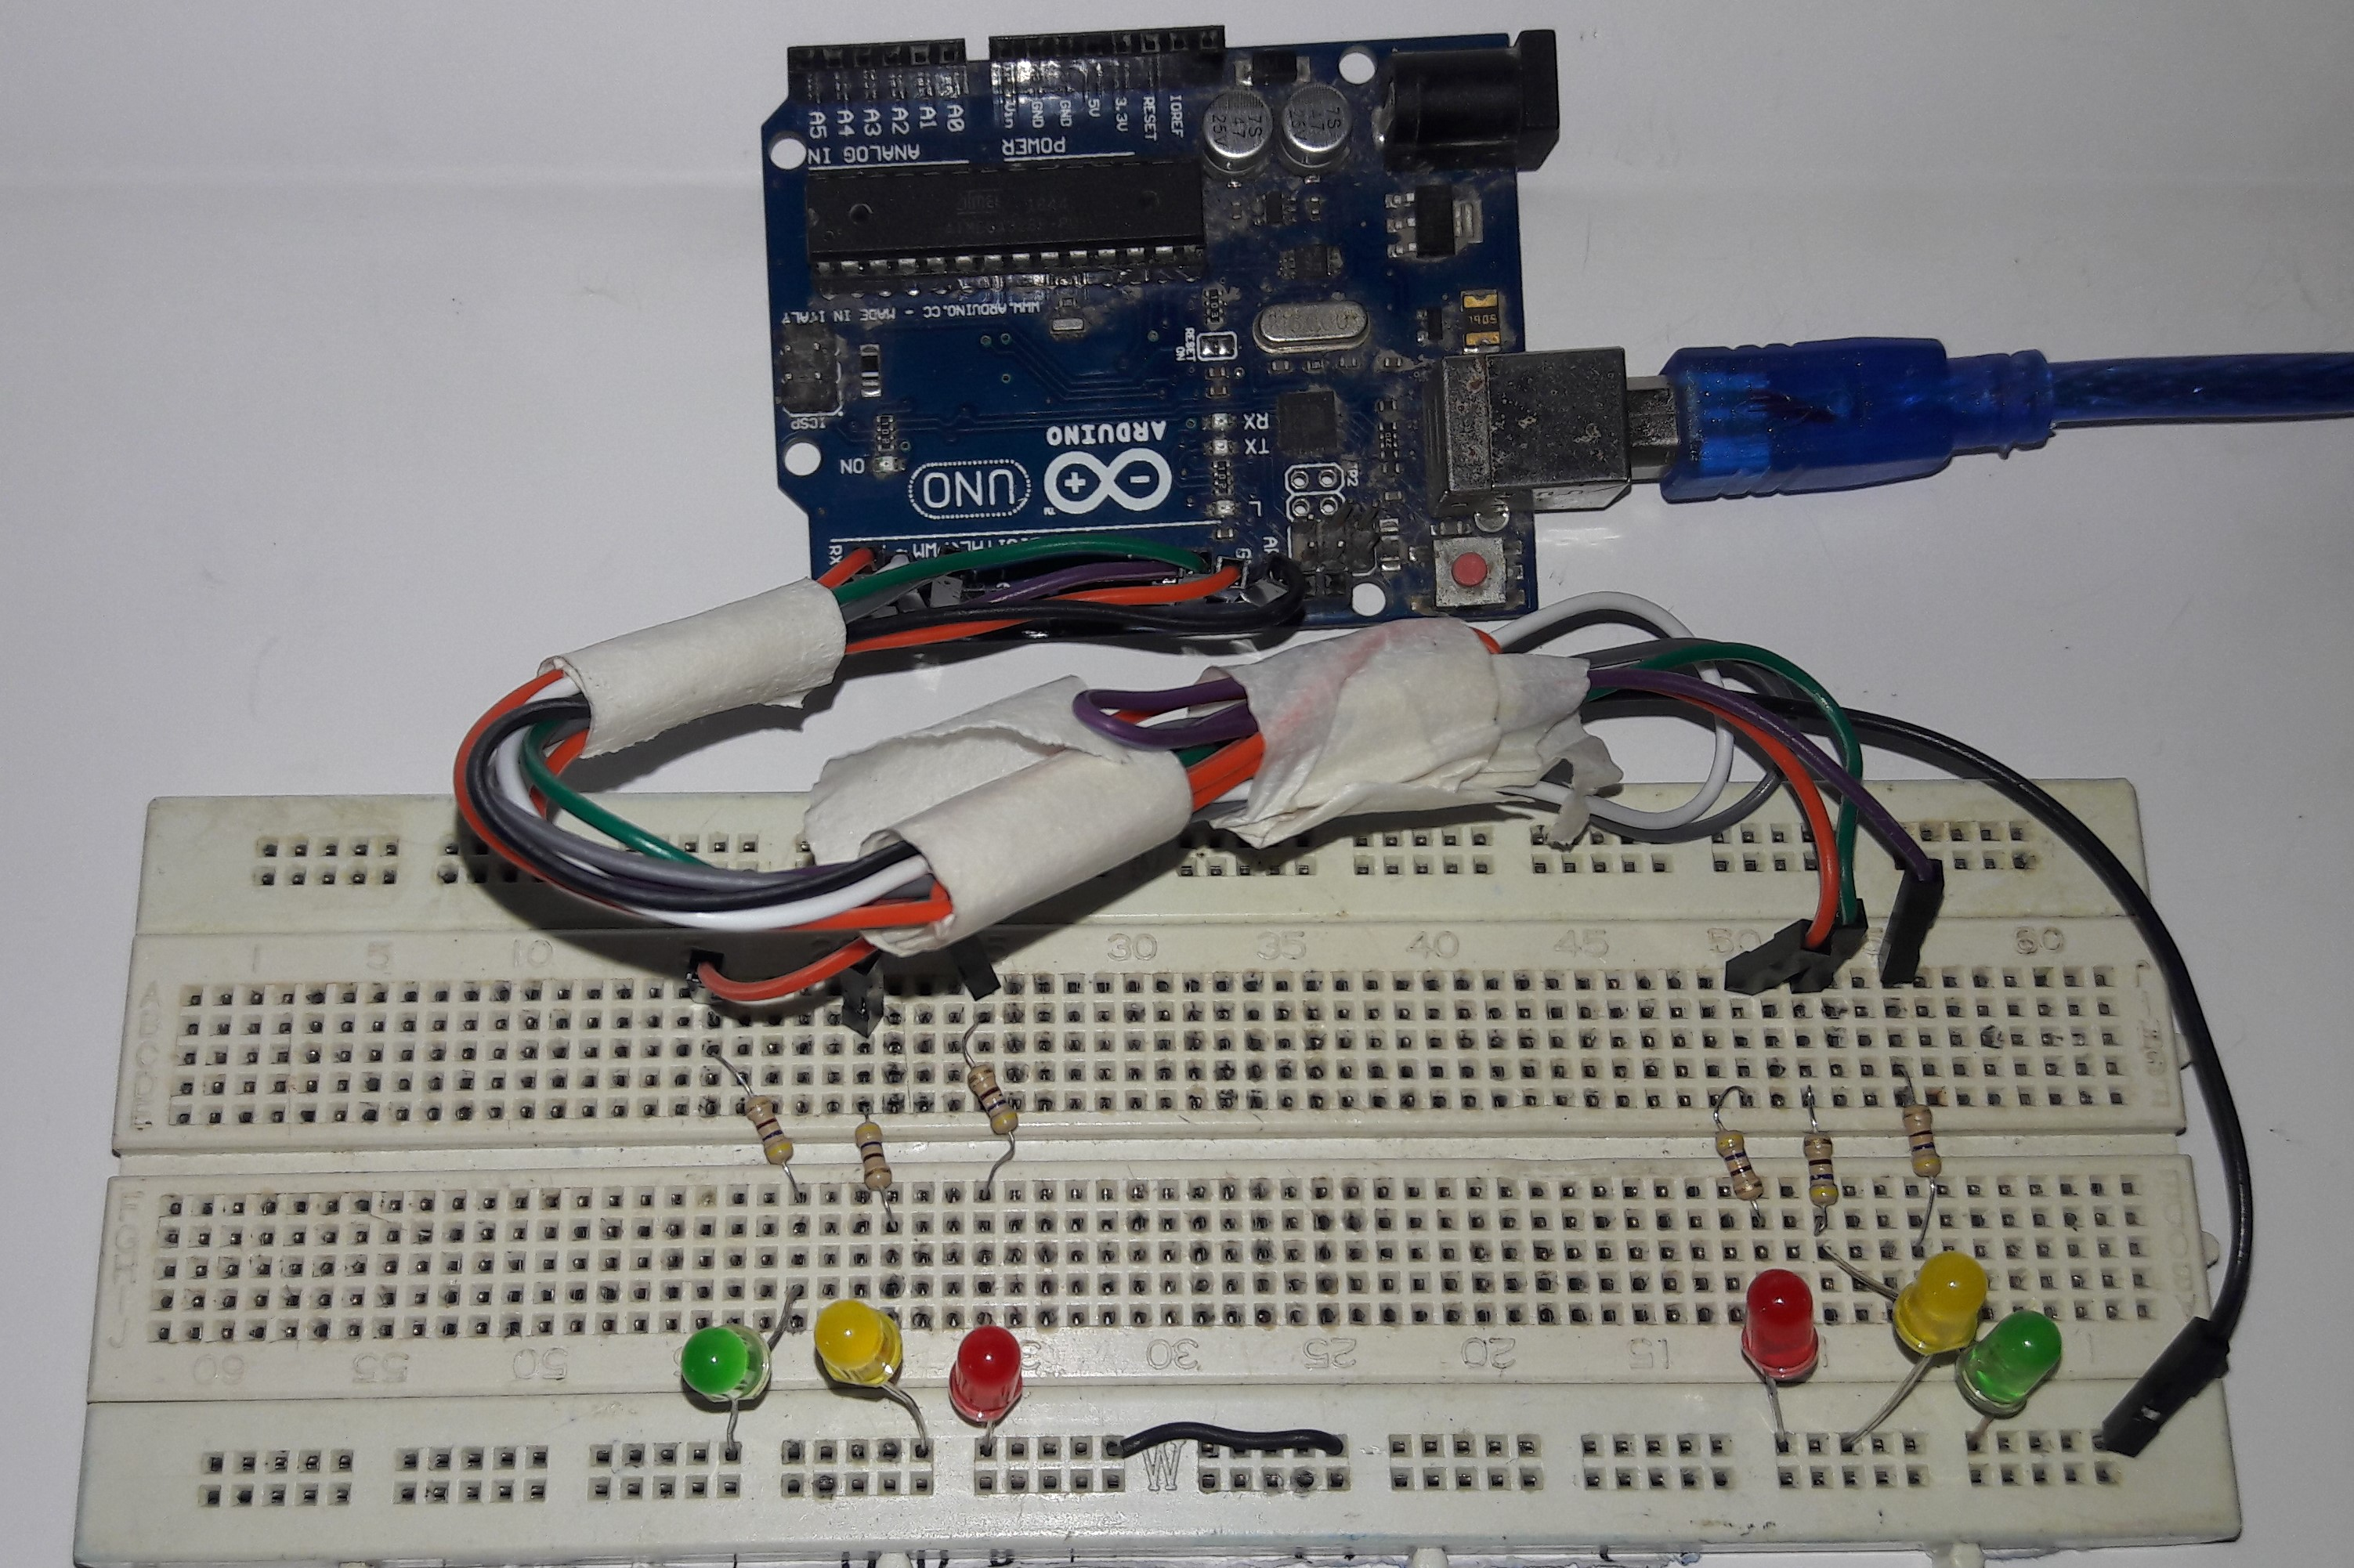
\includegraphics[width=0.5\linewidth]{recreational_exp/experiment_pics/traffic light.jpg}
	\caption{Hardware of the experiment}
\end{figure}
